%%%%%%%%%%%%%%%%%%%%%%%%%%%%%%%%%%%%%%%%%
% baposter Portrait Poster
% LaTeX Template
% Version 1.0 (15/5/13)
%
% Created by:
% Brian Amberg (baposter@brian-amberg.de)
%
% This template has been downloaded from:
% http://www.LaTeXTemplates.com
%
% License:
% CC BY-NC-SA 3.0 (http://creativecommons.org/licenses/by-nc-sa/3.0/)
%
%%%%%%%%%%%%%%%%%%%%%%%%%%%%%%%%%%%%%%%%%

%----------------------------------------------------------------------------------------
%	PACKAGES AND OTHER DOCUMENT CONFIGURATIONS
%----------------------------------------------------------------------------------------

\documentclass[a0paper,portrait]{baposter}

\usepackage[font=small,labelfont=bf]{caption} % Required for specifying captions to tables and figures
\usepackage{booktabs} % Horizontal rules in tables
\usepackage{relsize} % Used for making text smaller in some places
\usepackage{url}
\usepackage{multirow}
\usepackage{multicol}

\graphicspath{{figures/}} % Directory in which figures are stored

\definecolor{bordercol}{RGB}{40,40,40} % Border color of content boxes
\definecolor{headercol1}{RGB}{186,215,230} % Background color for the header in the content boxes (left side)
\definecolor{headercol2}{RGB}{80,80,80} % Background color for the header in the content boxes (right side)
\definecolor{headerfontcol}{RGB}{0,0,0} % Text color for the header text in the content boxes
\definecolor{boxcolor}{RGB}{186,215,230} % Background color for the content in the content boxes
\definecolor{emphsizecol}{RGB}{250,85,10} % Contrast color
\definecolor{contrastcol}{RGB}{0,200,0} % Contrast color

\begin{document}

\background{ % Set the background to an image (background.pdf)
\begin{tikzpicture}[remember picture,overlay]
\draw (current page.north west)+(-2em,2em) node[anchor=north west]
{\includegraphics[height=1.1\textheight]{background}};
\end{tikzpicture}
}

\begin{poster}{
grid=false,
borderColor=bordercol, % Border color of content boxes
headerColorOne=headercol1, % Background color for the header in the content boxes (left side)
headerColorTwo=headercol2, % Background color for the header in the content boxes (right side)
headerFontColor=headerfontcol, % Text color for the header text in the content boxes
boxColorOne=boxcolor, % Background color for the content in the content boxes
headershape=roundedright, % Specify the rounded corner in the content box headers
headerfont=\Large\sf\bf, % Font modifiers for the text in the content box headers
textborder=rectangle,
background=user,
headerborder=open, % Change to closed for a line under the content box headers
boxshade=plain
}
{}
%
%----------------------------------------------------------------------------------------
%	TITLE AND AUTHOR NAME
%----------------------------------------------------------------------------------------
%
{\sf\bf \LARGE{Sammba-MRI: SmAll MaMmals BrAin MRI in Python}} % Poster title
{\vspace{1em} Salma Bougacha{\textsuperscript{1,2}}, Nachiket Nadkarni\textsuperscript{1}, Cl\'ement Garin\textsuperscript{1}, Marc Dhenain\textsuperscript{1}\\ % Author names
{\small 1  Neurodegenerative Dis. Lab., MIRCen, CEA, Fontenay aux Roses Cedex, France;
2  U1077, INSERM, Caen, France}} % Author email addresses
{
\includegraphics[scale=0.4]{cyceron_mircen.png}} % University/lab logo

%----------------------------------------------------------------------------------------
%	INTRODUCTION
%----------------------------------------------------------------------------------------

\headerbox{Introduction}{name=introduction,column=0,row=0}{

The available software for processing small mammals neuroimaging data lacks maturity:

\begin{itemize}
\item Active efforts for Bruker format handling
\item Usual manual initialization for registration
\item Processing failure is not uncommon
%depending on the images quality
\end{itemize}

sammba-MRI
enables  \textcolor{emphsizecol}{\textbf{fluent scriptable}} analysis workflows, from DICOM conversion to results visualization.

}

%----------------------------------------------------------------------------------------
%	DATA
%----------------------------------------------------------------------------------------

\headerbox{Data}{name=data,column=0,below=introduction}{

4 Bruker datasets have been used

\begin{center}
\begin{tabular}{c c c}
\toprule
\textbf{Dataset} & \textbf{Animals} & \textbf{scans} \\
\midrule
Brookhaven's  			& 12 C57 mice 		& anat T2 			  \\ %BL/6J, Bruker 9.4 T
database \cite{ma:2008}  & 3-4 months 		&					 	    \\%12-14 weeks
	 	  			&					&							\\
Inhouse 1 \cite{nadkarni:2017}  & 34 lemurs 		& anat T2 			\\% Bruker 11.7 T
	  &	15-60 months  	&							\\
	 	  &					&							\\
Inhouse	2  &	10 C57 mice 		& anat T2  			\\% Bruker 11.7 T
	  	  & 5-7 months 		& perfusion			  		\\
	 	  &					&							\\
Zurich test-	  & 15 C57 mice 		& anat T2 			 \\% Bruker 9.4 T
retest data \cite{zerbi:2015}  	  & 2-3 months  	& BOLD-EPI   		 		\\
\bottomrule
\end{tabular}
%\captionof{table}{Data characteristics}
\end{center}
 
}

%----------------------------------------------------------------------------------------
%	MATERIAL AND METHODS
%----------------------------------------------------------------------------------------

\headerbox{Materials and Methods}{name=methods,column=0,below=data}{

Sammba-MRI  provides end-to-end pipelines to process and analyze multimodal images.
It combines functionalities from various existing software packages to tackle small animal processing difficulties.

Sammba-MRI allows to:

\begin{itemize}
\item \textcolor{emphsizecol}{\textbf{convert Bruker}} DICOM files to NIFTI-1
\item \textcolor{emphsizecol}{\textbf{perform registration}} by using ANTS, AFNI, FSL and RATS  \cite{yin:2010, oguz:2014}, all 
leveraged  through nipype  \cite{gorgolewski:2011}
\item \textcolor{emphsizecol}{\textbf{estimate perfusion}} maps for FAIR EPI sequences
\end{itemize}

Resting  state fMRI (rsfMRI) \textcolor{emphsizecol}{\textbf{connectivity analysis}} and brain images \textcolor{emphsizecol}{\textbf{visualization}} are straightforward with nilearn  \cite{abraham:2014} once the registration is performed.


}

%----------------------------------------------------------------------------------------
%	REFERENCES
%----------------------------------------------------------------------------------------

\headerbox{References}{name=references,column=0,below=methods, above=bottom}{

%\smaller % Reduce the font size in this block

\renewcommand{\section}[2]{\vskip 0.05em} % Get rid of the default "References" section title
\nocite{*} % Insert publications even if they are not cited in the poster

\bibliographystyle{unsrt}
\tiny{\bibliography{sample}} % Use sample.bib as the bibliography file
}

%----------------------------------------------------------------------------------------
%	RESULTS 1
%----------------------------------------------------------------------------------------

\headerbox{Results 1: Registration accuracy}{name=results1,span=2,column=1,row=0}{ % To reduce this block to 1 column width, remove 'span=2'
\begin{minipage}[t]{0.45\textwidth}
Registration accuracy has been evaluated on Brookhaven's data \cite{ma:2008} by measuring the correspondence of segmented structures between individual images registered 
to their average template and the template itself.
Because the shared individual images have been pre-registered to one reference image, they have been submitted to slight random quadratic deformations\footnote{Normally distributed coefficients with std=$0.1$ mm for translation, $0.1$ degrees for rotation, $0.02$ mm for scaling, $0.02$ mm for shear and $0.005$ mm for the remaining $31$ polynomial coefficients.} before performing registration.

For comparison purposes, registration has been repeated using SPM mouse \cite{sawiak:2009}.
Regional overlap was measured
%between each region in the average atlas and the transformed mice atlases 
using Dice's coefficient.
Figure 1 shows that sammba-MRI registration achieves
high overlap values and outperforms SPM mouse in the majority of cases.
\end{minipage}\hspace{.2em}
\begin{minipage}[t]{0.54\textwidth}
\begin{center}
\label{fig:dice}
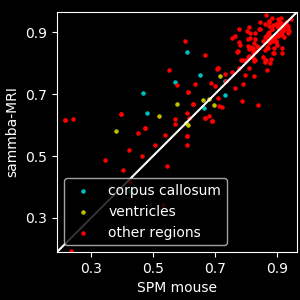
\includegraphics[height=.12\textheight]{bil2_transfo_dice_boxplots.png}
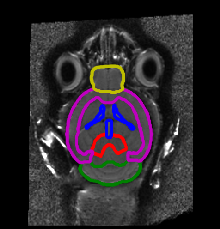
\includegraphics[height=.12\textheight]{atlas_overlays_dim-1pt6.png}
\captionof{figure}{Dice's coefficient per region and animal (left); typical registered mouse image with average atlas contours superimposed as coloured lines (right).}
\end{center}
\end{minipage}


%------------------------------------------------




}

%----------------------------------------------------------------------------------------
%	RESULTS 2
%----------------------------------------------------------------------------------------

\headerbox{Results 2: Group studies}{name=results2,span=2,column=1,below=results1}{ % To reduce this block to 1 column width, remove 'span=2'
\begin{minipage}[t]{0.55\textwidth}
\textbf{\large{\textcolor{contrastcol}{Template creation}}}
Studying   populations   of   animals   gains   precision   via   the   use   of   cohort   specific   templates.  
Sammba-MRI   proposes   an   iterative   method   to   create   a   fine   anatomical   template   from   individual  
structural   MRI   scans.   We   show   in   Figure 2 the template  created   from   34   mouse  
lemurs (inhouse dataset 1 \cite{nadkarni:2017}). The method adapts to different animal species.
\end{minipage}\hspace{1em}
\begin{minipage}[t]{0.4\textwidth}
\begin{center}
\label{fig:template}
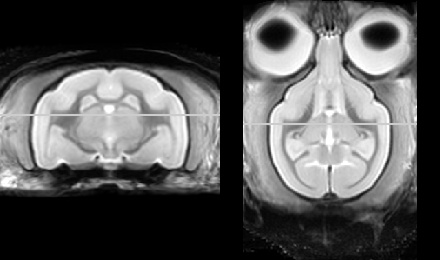
\includegraphics[width=.95\linewidth]{sfn_template.jpg}
\captionof{figure}{mouse lemur template}
\end{center}
\end{minipage}


%------------------------------------------------
\textbf{\large{\textcolor{contrastcol}{Cerebral blood flow quantification}}}
Estimating   the   cerebral   blood   flow   (CBF)   in   animals   is   challenging   due   to   the   low   SNR   and   lack   of  
sensitivity.   Sammba-MRI   allows   to   estimate   quantitative   CBF   maps   for   Bruker-FAIR   EPI  
sequences. Figure 3 shows voxelwise map and regional absolute CBF values from a group of 10 mice (inhouse dataset 2), all in agreement with the literature.

%------------------------------------------------
\begin{center}
\label{fig:cbf}
\includegraphics[height=.1\textheight]{mean_cbf_mricron2.png}
\hspace{3em}
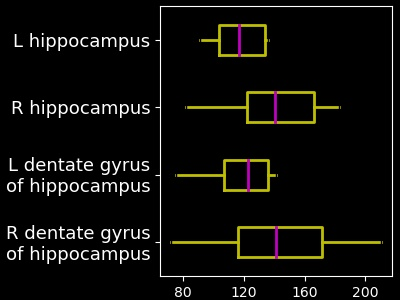
\includegraphics[height=.1\textheight]{regional_cbf_4rois_black_bg.jpg}
\captionof{figure}{Group   average   CBF   map (left); individual regional CBF in ml/100g/min (right)}
\end{center}

%------------------------------------------------
\textbf{\large\textcolor{contrastcol}{{Resting state networks}}}
Resting   state   spatial   networks   extraction   can   be   achieved through   independent components analysis (ICA). We  
performed   ICA  with nilearn on   a   group   of   15   mice (Zurich dataset \cite{zerbi:2015})  after registering functional images to a common space
with sammba-MRI.   Relevant   bilateral  
regions are found even without data post-processing (Figure 4).

%------------------------------------------------
\begin{center}
\includegraphics[width=0.17\linewidth]{{component1.jpg}}
\includegraphics[width=0.17\linewidth]{{component5.jpg}}
\includegraphics[width=0.17\linewidth]{{component9.jpg}}
\includegraphics[width=0.17\linewidth]{{component10.jpg}}
\includegraphics[width=0.17\linewidth]{{component13.jpg}}
\includegraphics[width=0.17\linewidth]{{component16.jpg}}
\includegraphics[width=0.17\linewidth]{{component17.jpg}}
\includegraphics[width=0.17\linewidth]{{component21.jpg}}
\includegraphics[width=0.17\linewidth]{{component26.jpg}}
\captionof{figure}{Bilateral ICA components}
\end{center}
}
%----------------------------------------------------------------------------------------
%	RESULTS 2
%----------------------------------------------------------------------------------------

\headerbox{Highlights}{name=conclusion,span=2,column=1,below=results2,above=bottom}{

\begin{minipage}[t]{0.5\textwidth}
\textbf{Multimodal, multispecies}\\
\textbf{Demos on public small animal data}
\end{minipage}
\begin{minipage}[t]{0.5\textwidth}
\textbf{Optimized pipeline rerunning}\\
\textbf{Parallelization}
\end{minipage}

%------------------------------------------------

\begin{center}
\textbf{\Large{\textcolor{emphsizecol}{\textbf{\url{https://sammba-mri.github.io}}}}}
\end{center}
}

%----------------------------------------------------------------------------------------

\end{poster}

\end{document}